\begin{figure}[h] 
\centering 
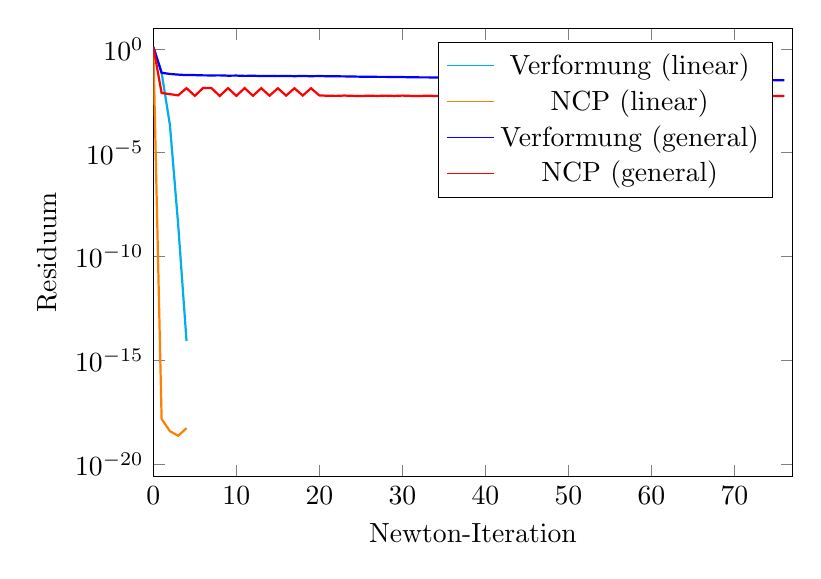
\begin{tikzpicture}[every plot/.append style={thick}] 
\begin{axis}[ 
label style={font=\normalsize}, 
xlabel={Newton-Iteration}, 
ylabel={Residuum}, 
xmin=0, xmax=77, 
ymode=log, 
ymin=0, ymax=10, 
width=0.8\textwidth, 
height=0.6\textwidth, 
legend pos=north east, 
legend style={cells={align=left}}, 
grid style=dashed, 
] 
\addplot[ 
color=cyan, 
] 
coordinates { 
(0, 1.25e+00)(1, 7.14e-02)(2, 2.19e-04)(3, 3.22e-09)(4, 8.53e-15)}; 
\addlegendentry{Verformung (linear)} 
\addplot[ 
color=orange, 
] 
coordinates { 
(0, 1.26e+00)(1, 1.49e-18)(2, 3.83e-19)(3, 2.30e-19)(4, 5.37e-19)}; 
\addlegendentry{NCP (linear)} 
\addplot[ 
color=blue, 
] 
coordinates { 
(0, 1.25e+00)(1, 7.14e-02)(2, 6.25e-02)(3, 5.81e-02)(4, 5.53e-02)(5, 5.51e-02)(6, 5.35e-02)(7, 5.32e-02)(8, 5.35e-02)(9, 5.17e-02)(10, 5.22e-02)(11, 5.05e-02)(12, 5.12e-02)(13, 4.97e-02)(14, 5.05e-02)(15, 4.92e-02)(16, 5.00e-02)(17, 4.89e-02)(18, 4.98e-02)(19, 4.87e-02)(20, 4.97e-02)(21, 4.87e-02)(22, 4.80e-02)(23, 4.79e-02)(24, 4.69e-02)(25, 4.63e-02)(26, 4.62e-02)(27, 4.53e-02)(28, 4.53e-02)(29, 4.44e-02)(30, 4.43e-02)(31, 4.35e-02)(32, 4.29e-02)(33, 4.29e-02)(34, 4.21e-02)(35, 4.21e-02)(36, 4.13e-02)(37, 4.13e-02)(38, 4.05e-02)(39, 4.00e-02)(40, 4.01e-02)(41, 3.93e-02)(42, 3.94e-02)(43, 3.87e-02)(44, 3.87e-02)(45, 3.81e-02)(46, 3.76e-02)(47, 3.77e-02)(48, 3.70e-02)(49, 3.71e-02)(50, 3.65e-02)(51, 3.66e-02)(52, 3.60e-02)(53, 3.61e-02)(54, 3.55e-02)(55, 3.51e-02)(56, 3.53e-02)(57, 3.47e-02)(58, 3.48e-02)(59, 3.43e-02)(60, 3.44e-02)(61, 3.39e-02)(62, 3.35e-02)(63, 3.37e-02)(64, 3.31e-02)(65, 3.33e-02)(66, 3.28e-02)(67, 3.30e-02)(68, 3.25e-02)(69, 3.21e-02)(70, 3.23e-02)(71, 3.19e-02)(72, 3.21e-02)(73, 3.16e-02)(74, 3.18e-02)(75, 3.14e-02)(76, 3.10e-02)}; 
\addlegendentry{Verformung (general)} 
\addplot[ 
color=red, 
] 
coordinates { 
(0, 1.26e+00)(1, 7.61e-03)(2, 6.66e-03)(3, 5.83e-03)(4, 1.30e-02)(5, 5.51e-03)(6, 1.33e-02)(7, 1.31e-02)(8, 5.43e-03)(9, 1.30e-02)(10, 5.50e-03)(11, 1.30e-02)(12, 5.56e-03)(13, 1.29e-02)(14, 5.62e-03)(15, 1.28e-02)(16, 5.67e-03)(17, 1.28e-02)(18, 5.71e-03)(19, 1.28e-02)(20, 5.76e-03)(21, 5.58e-03)(22, 5.49e-03)(23, 5.69e-03)(24, 5.51e-03)(25, 5.42e-03)(26, 5.62e-03)(27, 5.45e-03)(28, 5.65e-03)(29, 5.47e-03)(30, 5.67e-03)(31, 5.49e-03)(32, 5.41e-03)(33, 5.61e-03)(34, 5.43e-03)(35, 5.63e-03)(36, 5.45e-03)(37, 5.65e-03)(38, 5.48e-03)(39, 5.39e-03)(40, 5.59e-03)(41, 5.42e-03)(42, 5.62e-03)(43, 5.44e-03)(44, 5.64e-03)(45, 5.46e-03)(46, 5.38e-03)(47, 5.58e-03)(48, 5.40e-03)(49, 5.60e-03)(50, 5.43e-03)(51, 5.63e-03)(52, 5.45e-03)(53, 5.65e-03)(54, 5.47e-03)(55, 5.39e-03)(56, 5.59e-03)(57, 5.41e-03)(58, 5.61e-03)(59, 5.44e-03)(60, 5.64e-03)(61, 5.46e-03)(62, 5.38e-03)(63, 5.58e-03)(64, 5.40e-03)(65, 5.60e-03)(66, 5.43e-03)(67, 5.63e-03)(68, 5.45e-03)(69, 5.37e-03)(70, 5.57e-03)(71, 5.39e-03)(72, 5.59e-03)(73, 5.42e-03)(74, 5.62e-03)(75, 5.44e-03)(76, 5.36e-03)}; 
\addlegendentry{NCP (general)} 
\end{axis} 
\end{tikzpicture} 
\caption{Residuen des Stoffgesetzes 'Neo Hooke' mit Hinderniss 'Hut' und 578 Freiheitsgraden für die Verschiebung.} 
\label{fiq:NeoHooke_Hut_level3} 
\end{figure} 
